\documentclass[twoside]{book}

% Packages required by doxygen
\usepackage{fixltx2e}
\usepackage{calc}
\usepackage{doxygen}
\usepackage{graphicx}
\usepackage[utf8]{inputenc}
\usepackage{makeidx}
\usepackage{multicol}
\usepackage{multirow}
\PassOptionsToPackage{warn}{textcomp}
\usepackage{textcomp}
\usepackage[nointegrals]{wasysym}
\usepackage[table]{xcolor}

% Font selection
\usepackage[T1]{fontenc}
\usepackage{mathptmx}
\usepackage[scaled=.90]{helvet}
\usepackage{courier}
\usepackage{amssymb}
\usepackage{sectsty}
\renewcommand{\familydefault}{\sfdefault}
\allsectionsfont{%
  \fontseries{bc}\selectfont%
  \color{darkgray}%
}
\renewcommand{\DoxyLabelFont}{%
  \fontseries{bc}\selectfont%
  \color{darkgray}%
}
\newcommand{\+}{\discretionary{\mbox{\scriptsize$\hookleftarrow$}}{}{}}

% Page & text layout
\usepackage{geometry}
\geometry{%
  a4paper,%
  top=2.5cm,%
  bottom=2.5cm,%
  left=2.5cm,%
  right=2.5cm%
}
\tolerance=750
\hfuzz=15pt
\hbadness=750
\setlength{\emergencystretch}{15pt}
\setlength{\parindent}{0cm}
\setlength{\parskip}{0.2cm}
\makeatletter
\renewcommand{\paragraph}{%
  \@startsection{paragraph}{4}{0ex}{-1.0ex}{1.0ex}{%
    \normalfont\normalsize\bfseries\SS@parafont%
  }%
}
\renewcommand{\subparagraph}{%
  \@startsection{subparagraph}{5}{0ex}{-1.0ex}{1.0ex}{%
    \normalfont\normalsize\bfseries\SS@subparafont%
  }%
}
\makeatother

% Headers & footers
\usepackage{fancyhdr}
\pagestyle{fancyplain}
\fancyhead[LE]{\fancyplain{}{\bfseries\thepage}}
\fancyhead[CE]{\fancyplain{}{}}
\fancyhead[RE]{\fancyplain{}{\bfseries\leftmark}}
\fancyhead[LO]{\fancyplain{}{\bfseries\rightmark}}
\fancyhead[CO]{\fancyplain{}{}}
\fancyhead[RO]{\fancyplain{}{\bfseries\thepage}}
\fancyfoot[LE]{\fancyplain{}{}}
\fancyfoot[CE]{\fancyplain{}{}}
\fancyfoot[RE]{\fancyplain{}{\bfseries\scriptsize Generated on Tue Nov 29 2016 15\+:21\+:51 for G\+O\+A\+P A\+I by Doxygen }}
\fancyfoot[LO]{\fancyplain{}{\bfseries\scriptsize Generated on Tue Nov 29 2016 15\+:21\+:51 for G\+O\+A\+P A\+I by Doxygen }}
\fancyfoot[CO]{\fancyplain{}{}}
\fancyfoot[RO]{\fancyplain{}{}}
\renewcommand{\footrulewidth}{0.4pt}
\renewcommand{\chaptermark}[1]{%
  \markboth{#1}{}%
}
\renewcommand{\sectionmark}[1]{%
  \markright{\thesection\ #1}%
}

% Indices & bibliography
\usepackage{natbib}
\usepackage[titles]{tocloft}
\setcounter{tocdepth}{3}
\setcounter{secnumdepth}{5}
\makeindex

% Hyperlinks (required, but should be loaded last)
\usepackage{ifpdf}
\ifpdf
  \usepackage[pdftex,pagebackref=true]{hyperref}
\else
  \usepackage[ps2pdf,pagebackref=true]{hyperref}
\fi
\hypersetup{%
  colorlinks=true,%
  linkcolor=blue,%
  citecolor=blue,%
  unicode%
}

% Custom commands
\newcommand{\clearemptydoublepage}{%
  \newpage{\pagestyle{empty}\cleardoublepage}%
}


%===== C O N T E N T S =====

\begin{document}

% Titlepage & ToC
\hypersetup{pageanchor=false,
             bookmarks=true,
             bookmarksnumbered=true,
             pdfencoding=unicode
            }
\pagenumbering{roman}
\begin{titlepage}
\vspace*{7cm}
\begin{center}%
{\Large G\+O\+A\+P A\+I \\[1ex]\large Release Candidate 1 }\\
\vspace*{1cm}
{\large Generated by Doxygen 1.8.8}\\
\vspace*{0.5cm}
{\small Tue Nov 29 2016 15:21:51}\\
\end{center}
\end{titlepage}
\clearemptydoublepage
\tableofcontents
\clearemptydoublepage
\pagenumbering{arabic}
\hypersetup{pageanchor=true}

%--- Begin generated contents ---
\chapter{Hierarchical Index}
\section{Class Hierarchy}
This inheritance list is sorted roughly, but not completely, alphabetically\+:\begin{DoxyCompactList}
\item \contentsline{section}{F\+S\+M}{\pageref{class_f_s_m}}{}
\item \contentsline{section}{F\+S\+M\+State}{\pageref{interface_f_s_m_state}}{}
\item \contentsline{section}{I\+Goap}{\pageref{interface_i_goap}}{}
\item Mono\+Behaviour\begin{DoxyCompactList}
\item \contentsline{section}{Action}{\pageref{class_action}}{}
\item \contentsline{section}{Goal}{\pageref{class_goal}}{}
\item \contentsline{section}{G\+O\+A\+P}{\pageref{class_g_o_a_p}}{}
\item \contentsline{section}{Goap\+Agent}{\pageref{class_goap_agent}}{}
\item \contentsline{section}{G\+O\+A\+P\+Planner}{\pageref{class_g_o_a_p_planner}}{}
\end{DoxyCompactList}
\end{DoxyCompactList}

\chapter{Class Index}
\section{Class List}
Here are the classes, structs, unions and interfaces with brief descriptions\+:\begin{DoxyCompactList}
\item\contentsline{section}{\hyperlink{class_action}{Action} \\*A \hyperlink{class_g_o_a_p}{G\+O\+A\+P} action can have a set of requirements and a cost, it then has an effect when completed so that the planner can use it to satisfy a \hyperlink{class_goal}{Goal} }{\pageref{class_action}}{}
\item\contentsline{section}{\hyperlink{class_f_s_m}{F\+S\+M} \\*the \hyperlink{class_f_s_m}{F\+S\+M} class covers the bare minimum to provide \hyperlink{class_g_o_a_p}{G\+O\+A\+P} Agents with a way to transition between the 3 main states\+: Idle Move Perform }{\pageref{class_f_s_m}}{}
\item\contentsline{section}{\hyperlink{interface_f_s_m_state}{F\+S\+M\+State} \\*An interface for concrete implemetations of \hyperlink{class_f_s_m}{F\+S\+M} states }{\pageref{interface_f_s_m_state}}{}
\item\contentsline{section}{\hyperlink{class_goal}{Goal} }{\pageref{class_goal}}{}
\item\contentsline{section}{\hyperlink{class_g_o_a_p}{G\+O\+A\+P} }{\pageref{class_g_o_a_p}}{}
\item\contentsline{section}{\hyperlink{class_goap_agent}{Goap\+Agent} }{\pageref{class_goap_agent}}{}
\item\contentsline{section}{\hyperlink{class_g_o_a_p_planner}{G\+O\+A\+P\+Planner} \\*The Planner takes care of providing each agent with a queue of actions that they can perform to achieve their goal. The following code has been copied as is from \href{https://github.com/sploreg/goap/blob/master/Assets/Standard%20Assets/Scripts/AI/GOAP/GoapPlanner.cs}{\tt https\+://github.\+com/sploreg/goap/blob/master/\+Assets/\+Standard\%20\+Assets/\+Scripts/\+A\+I/\+G\+O\+A\+P/\+Goap\+Planner.\+cs}. This has been done as, after an analysys of the code, it was considered impossible to create a version of it that would do the same job in a significantly different way. Therefore the entirety of Brent Owens' code was just copied and refactored to integrate with the existing codebase. }{\pageref{class_g_o_a_p_planner}}{}
\item\contentsline{section}{\hyperlink{interface_i_goap}{I\+Goap} \\*Any agent that wants to use \hyperlink{class_g_o_a_p}{G\+O\+A\+P} must implement this interface. It provides information to the \hyperlink{class_g_o_a_p}{G\+O\+A\+P} planner so it can plan what actions to use. It also provides an interface for the planner to give feedback to the Agent and report success/failure. }{\pageref{interface_i_goap}}{}
\end{DoxyCompactList}

\chapter{Class Documentation}
\hypertarget{class_action}{}\section{Action Class Reference}
\label{class_action}\index{Action@{Action}}


A \hyperlink{class_g_o_a_p}{G\+O\+A\+P} action can have a set of requirements and a cost, it then has an effect when completed so that the planner can use it to satisfy a \hyperlink{class_goal}{Goal}  


Inheritance diagram for Action\+:\begin{figure}[H]
\begin{center}
\leavevmode
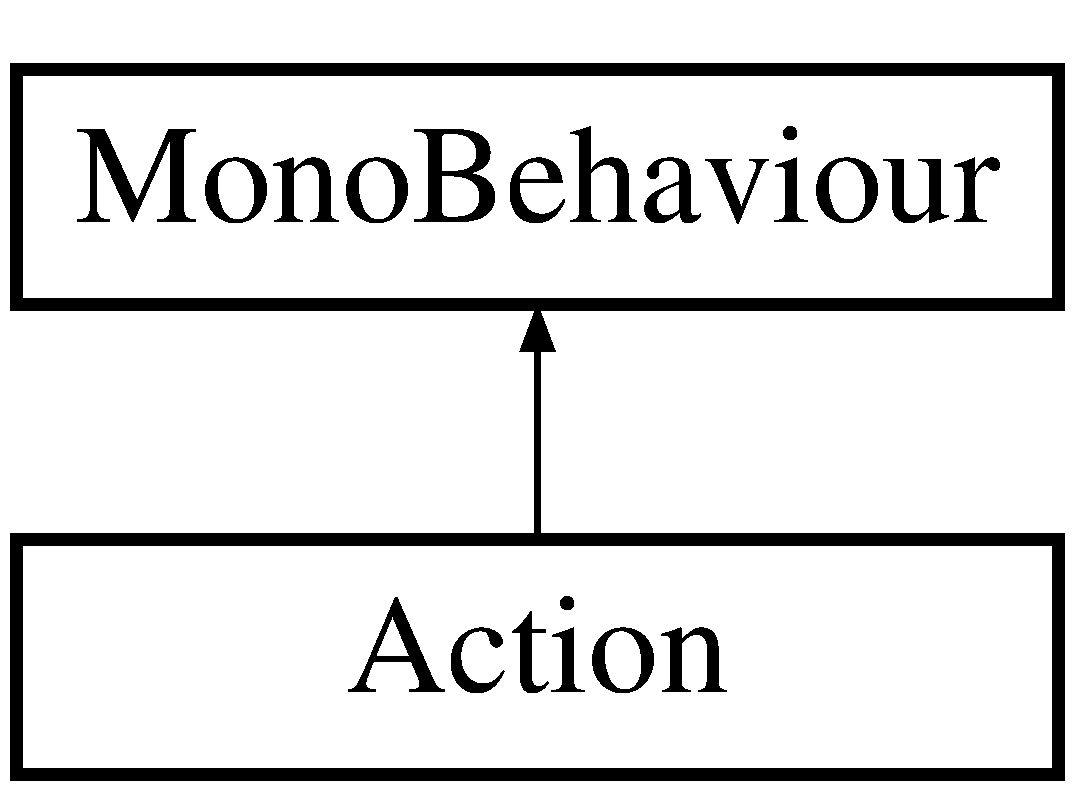
\includegraphics[height=2.000000cm]{class_action}
\end{center}
\end{figure}
\subsection*{Public Member Functions}
\begin{DoxyCompactItemize}
\item 
\hyperlink{class_action_aed886910937b93b956b61cff7be572bc}{Action} ()
\begin{DoxyCompactList}\small\item\em default constructor, initialises preconditions and effects \end{DoxyCompactList}\item 
void \hyperlink{class_action_a21740ddc42a7c47572caede717005763}{Do\+Reset} ()
\begin{DoxyCompactList}\small\item\em resets the action to its default state \end{DoxyCompactList}\item 
\hypertarget{class_action_ac1fbcc1054f462ea4e46aecec983e8ec}{}abstract void {\bfseries Reset} ()\label{class_action_ac1fbcc1054f462ea4e46aecec983e8ec}

\item 
\hypertarget{class_action_ada6d09848fa150cc89745fff1bc8b2d5}{}abstract bool {\bfseries Is\+Done} ()\label{class_action_ada6d09848fa150cc89745fff1bc8b2d5}

\item 
\hypertarget{class_action_a43360ddabf1415318e453fcaf9805c8d}{}abstract bool {\bfseries Check\+Procedural\+Precondition} (Game\+Object agent)\label{class_action_a43360ddabf1415318e453fcaf9805c8d}

\item 
\hypertarget{class_action_af779fa1eb5494513e7afe3450362f23e}{}abstract bool {\bfseries Perform} (Game\+Object agent)\label{class_action_af779fa1eb5494513e7afe3450362f23e}

\item 
\hypertarget{class_action_ac2df69ba49c45fc4fbd9f76e7c3beb56}{}abstract bool {\bfseries Requires\+In\+Range} ()\label{class_action_ac2df69ba49c45fc4fbd9f76e7c3beb56}

\item 
byte \hyperlink{class_action_ac1cd1bb574e98e9e299e786727395b93}{Get\+Cost} ()
\begin{DoxyCompactList}\small\item\em gets the cost of the action \end{DoxyCompactList}\item 
void \hyperlink{class_action_ad95984cfd81dd0debd89b2eb62f66d5f}{Set\+Cost} (byte cost)
\begin{DoxyCompactList}\small\item\em sets the cost for the action \end{DoxyCompactList}\item 
void \hyperlink{class_action_a60832e6094bf58d56b86db14c0c86244}{Set\+In\+Range} ()
\begin{DoxyCompactList}\small\item\em sets the action to be in range \end{DoxyCompactList}\item 
bool \hyperlink{class_action_a2f1a8b4050f57bf34f6691c4403898bc}{Get\+In\+Range} ()
\begin{DoxyCompactList}\small\item\em gets wether the action is in range or not \end{DoxyCompactList}\item 
void \hyperlink{class_action_aca3de1e11c18edc715a3322bc01c1e91}{Set\+Target} (Game\+Object target)
\begin{DoxyCompactList}\small\item\em sets a target for the action \end{DoxyCompactList}\item 
Game\+Object \hyperlink{class_action_a1c21dae76e175d5921d012a56e34c8b7}{Get\+Target} ()
\begin{DoxyCompactList}\small\item\em gets the action's target \end{DoxyCompactList}\item 
void \hyperlink{class_action_acf226c4a5fac20e472678232b1677b44}{Add\+Precondition} (string str, object obj)
\begin{DoxyCompactList}\small\item\em adds a new precondition to the Hash\+Set \end{DoxyCompactList}\item 
void \hyperlink{class_action_aae731975d3759bbbd4a03ff12804fda5}{Remove\+Precondition} (string key)
\begin{DoxyCompactList}\small\item\em removes a precondition from the Hash\+Set \end{DoxyCompactList}\item 
\hypertarget{class_action_aa2843e05295e1cd9f321c4f32f70646e}{}Hash\+Set$<$ Key\+Value\+Pair$<$ string, object $>$ $>$ {\bfseries Get\+Preconditions} ()\label{class_action_aa2843e05295e1cd9f321c4f32f70646e}

\item 
void \hyperlink{class_action_aff6e57b63affca019682039119895ef9}{Add\+Effect} (string str, object obj)
\begin{DoxyCompactList}\small\item\em similarly to preconditions, it adds a new effect in the Hash\+Set \end{DoxyCompactList}\item 
void \hyperlink{class_action_ac00e1048ff1eb9315a28e6dc6cecaccd}{Remove\+Effect} (string key)
\begin{DoxyCompactList}\small\item\em removes an effect from the Hash\+Set \end{DoxyCompactList}\item 
\hypertarget{class_action_a5ac53d1cc348f1e131bd8ffa649cc217}{}Hash\+Set$<$ Key\+Value\+Pair$<$ string, object $>$ $>$ {\bfseries Get\+Effects} ()\label{class_action_a5ac53d1cc348f1e131bd8ffa649cc217}

\end{DoxyCompactItemize}


\subsection{Detailed Description}
A \hyperlink{class_g_o_a_p}{G\+O\+A\+P} action can have a set of requirements and a cost, it then has an effect when completed so that the planner can use it to satisfy a \hyperlink{class_goal}{Goal} 



\subsection{Constructor \& Destructor Documentation}
\hypertarget{class_action_aed886910937b93b956b61cff7be572bc}{}\index{Action@{Action}!Action@{Action}}
\index{Action@{Action}!Action@{Action}}
\subsubsection[{Action}]{\setlength{\rightskip}{0pt plus 5cm}Action.\+Action (
\begin{DoxyParamCaption}
{}
\end{DoxyParamCaption}
)\hspace{0.3cm}{\ttfamily [inline]}}\label{class_action_aed886910937b93b956b61cff7be572bc}


default constructor, initialises preconditions and effects 



\subsection{Member Function Documentation}
\hypertarget{class_action_aff6e57b63affca019682039119895ef9}{}\index{Action@{Action}!Add\+Effect@{Add\+Effect}}
\index{Add\+Effect@{Add\+Effect}!Action@{Action}}
\subsubsection[{Add\+Effect}]{\setlength{\rightskip}{0pt plus 5cm}void Action.\+Add\+Effect (
\begin{DoxyParamCaption}
\item[{string}]{str, }
\item[{object}]{obj}
\end{DoxyParamCaption}
)\hspace{0.3cm}{\ttfamily [inline]}}\label{class_action_aff6e57b63affca019682039119895ef9}


similarly to preconditions, it adds a new effect in the Hash\+Set 


\begin{DoxyParams}{Parameters}
{\em str} & name of the effect\\
\hline
{\em obj} & value of the effect, usually a bool\\
\hline
\end{DoxyParams}
\hypertarget{class_action_acf226c4a5fac20e472678232b1677b44}{}\index{Action@{Action}!Add\+Precondition@{Add\+Precondition}}
\index{Add\+Precondition@{Add\+Precondition}!Action@{Action}}
\subsubsection[{Add\+Precondition}]{\setlength{\rightskip}{0pt plus 5cm}void Action.\+Add\+Precondition (
\begin{DoxyParamCaption}
\item[{string}]{str, }
\item[{object}]{obj}
\end{DoxyParamCaption}
)\hspace{0.3cm}{\ttfamily [inline]}}\label{class_action_acf226c4a5fac20e472678232b1677b44}


adds a new precondition to the Hash\+Set 


\begin{DoxyParams}{Parameters}
{\em str} & the name of the precondition\\
\hline
{\em obj} & the value of the precondition, usually a bool\\
\hline
\end{DoxyParams}
\hypertarget{class_action_a21740ddc42a7c47572caede717005763}{}\index{Action@{Action}!Do\+Reset@{Do\+Reset}}
\index{Do\+Reset@{Do\+Reset}!Action@{Action}}
\subsubsection[{Do\+Reset}]{\setlength{\rightskip}{0pt plus 5cm}void Action.\+Do\+Reset (
\begin{DoxyParamCaption}
{}
\end{DoxyParamCaption}
)\hspace{0.3cm}{\ttfamily [inline]}}\label{class_action_a21740ddc42a7c47572caede717005763}


resets the action to its default state 

\hypertarget{class_action_ac1cd1bb574e98e9e299e786727395b93}{}\index{Action@{Action}!Get\+Cost@{Get\+Cost}}
\index{Get\+Cost@{Get\+Cost}!Action@{Action}}
\subsubsection[{Get\+Cost}]{\setlength{\rightskip}{0pt plus 5cm}byte Action.\+Get\+Cost (
\begin{DoxyParamCaption}
{}
\end{DoxyParamCaption}
)\hspace{0.3cm}{\ttfamily [inline]}}\label{class_action_ac1cd1bb574e98e9e299e786727395b93}


gets the cost of the action 

\begin{DoxyReturn}{Returns}

\end{DoxyReturn}
\hypertarget{class_action_a2f1a8b4050f57bf34f6691c4403898bc}{}\index{Action@{Action}!Get\+In\+Range@{Get\+In\+Range}}
\index{Get\+In\+Range@{Get\+In\+Range}!Action@{Action}}
\subsubsection[{Get\+In\+Range}]{\setlength{\rightskip}{0pt plus 5cm}bool Action.\+Get\+In\+Range (
\begin{DoxyParamCaption}
{}
\end{DoxyParamCaption}
)\hspace{0.3cm}{\ttfamily [inline]}}\label{class_action_a2f1a8b4050f57bf34f6691c4403898bc}


gets wether the action is in range or not 

\begin{DoxyReturn}{Returns}

\end{DoxyReturn}
\hypertarget{class_action_a1c21dae76e175d5921d012a56e34c8b7}{}\index{Action@{Action}!Get\+Target@{Get\+Target}}
\index{Get\+Target@{Get\+Target}!Action@{Action}}
\subsubsection[{Get\+Target}]{\setlength{\rightskip}{0pt plus 5cm}Game\+Object Action.\+Get\+Target (
\begin{DoxyParamCaption}
{}
\end{DoxyParamCaption}
)\hspace{0.3cm}{\ttfamily [inline]}}\label{class_action_a1c21dae76e175d5921d012a56e34c8b7}


gets the action's target 

\begin{DoxyReturn}{Returns}

\end{DoxyReturn}
\hypertarget{class_action_ac00e1048ff1eb9315a28e6dc6cecaccd}{}\index{Action@{Action}!Remove\+Effect@{Remove\+Effect}}
\index{Remove\+Effect@{Remove\+Effect}!Action@{Action}}
\subsubsection[{Remove\+Effect}]{\setlength{\rightskip}{0pt plus 5cm}void Action.\+Remove\+Effect (
\begin{DoxyParamCaption}
\item[{string}]{key}
\end{DoxyParamCaption}
)\hspace{0.3cm}{\ttfamily [inline]}}\label{class_action_ac00e1048ff1eb9315a28e6dc6cecaccd}


removes an effect from the Hash\+Set 


\begin{DoxyParams}{Parameters}
{\em key} & name of the effect to be removed\\
\hline
\end{DoxyParams}
\hypertarget{class_action_aae731975d3759bbbd4a03ff12804fda5}{}\index{Action@{Action}!Remove\+Precondition@{Remove\+Precondition}}
\index{Remove\+Precondition@{Remove\+Precondition}!Action@{Action}}
\subsubsection[{Remove\+Precondition}]{\setlength{\rightskip}{0pt plus 5cm}void Action.\+Remove\+Precondition (
\begin{DoxyParamCaption}
\item[{string}]{key}
\end{DoxyParamCaption}
)\hspace{0.3cm}{\ttfamily [inline]}}\label{class_action_aae731975d3759bbbd4a03ff12804fda5}


removes a precondition from the Hash\+Set 


\begin{DoxyParams}{Parameters}
{\em key} & the name of the precondition to be removed\\
\hline
\end{DoxyParams}
\hypertarget{class_action_ad95984cfd81dd0debd89b2eb62f66d5f}{}\index{Action@{Action}!Set\+Cost@{Set\+Cost}}
\index{Set\+Cost@{Set\+Cost}!Action@{Action}}
\subsubsection[{Set\+Cost}]{\setlength{\rightskip}{0pt plus 5cm}void Action.\+Set\+Cost (
\begin{DoxyParamCaption}
\item[{byte}]{cost}
\end{DoxyParamCaption}
)\hspace{0.3cm}{\ttfamily [inline]}}\label{class_action_ad95984cfd81dd0debd89b2eb62f66d5f}


sets the cost for the action 


\begin{DoxyParams}{Parameters}
{\em cost} & \\
\hline
\end{DoxyParams}
\hypertarget{class_action_a60832e6094bf58d56b86db14c0c86244}{}\index{Action@{Action}!Set\+In\+Range@{Set\+In\+Range}}
\index{Set\+In\+Range@{Set\+In\+Range}!Action@{Action}}
\subsubsection[{Set\+In\+Range}]{\setlength{\rightskip}{0pt plus 5cm}void Action.\+Set\+In\+Range (
\begin{DoxyParamCaption}
{}
\end{DoxyParamCaption}
)\hspace{0.3cm}{\ttfamily [inline]}}\label{class_action_a60832e6094bf58d56b86db14c0c86244}


sets the action to be in range 

\hypertarget{class_action_aca3de1e11c18edc715a3322bc01c1e91}{}\index{Action@{Action}!Set\+Target@{Set\+Target}}
\index{Set\+Target@{Set\+Target}!Action@{Action}}
\subsubsection[{Set\+Target}]{\setlength{\rightskip}{0pt plus 5cm}void Action.\+Set\+Target (
\begin{DoxyParamCaption}
\item[{Game\+Object}]{target}
\end{DoxyParamCaption}
)\hspace{0.3cm}{\ttfamily [inline]}}\label{class_action_aca3de1e11c18edc715a3322bc01c1e91}


sets a target for the action 


\begin{DoxyParams}{Parameters}
{\em target} & \\
\hline
\end{DoxyParams}


The documentation for this class was generated from the following file\+:\begin{DoxyCompactItemize}
\item 
Assets/\+Code/\+G\+O\+A\+P/Action.\+cs\end{DoxyCompactItemize}

\hypertarget{class_f_s_m}{}\section{F\+S\+M Class Reference}
\label{class_f_s_m}\index{F\+S\+M@{F\+S\+M}}


the \hyperlink{class_f_s_m}{F\+S\+M} class covers the bare minimum to provide \hyperlink{class_g_o_a_p}{G\+O\+A\+P} Agents with a way to transition between the 3 main states\+: Idle Move Perform  


\subsection*{Public Member Functions}
\begin{DoxyCompactItemize}
\item 
\hypertarget{class_f_s_m_a7c92cc5309ca4f83c8f7984579901996}{}delegate void {\bfseries F\+S\+M\+State} (\hyperlink{class_f_s_m}{F\+S\+M} fsm, Game\+Object game\+Object)\label{class_f_s_m_a7c92cc5309ca4f83c8f7984579901996}

\item 
\hypertarget{class_f_s_m_a5d544e5c245b1b90b78eb5b2951ba1da}{}void {\bfseries Update} (Game\+Object game\+Object)\label{class_f_s_m_a5d544e5c245b1b90b78eb5b2951ba1da}

\item 
\hypertarget{class_f_s_m_a150457bcd1fce2077d7260a46de403b2}{}void {\bfseries Push\+State} (\hyperlink{interface_f_s_m_state}{F\+S\+M\+State} state)\label{class_f_s_m_a150457bcd1fce2077d7260a46de403b2}

\item 
\hypertarget{class_f_s_m_af3ecd111eb7f58a2817e1e23960b6e58}{}void {\bfseries Pop\+State} ()\label{class_f_s_m_af3ecd111eb7f58a2817e1e23960b6e58}

\end{DoxyCompactItemize}


\subsection{Detailed Description}
the \hyperlink{class_f_s_m}{F\+S\+M} class covers the bare minimum to provide \hyperlink{class_g_o_a_p}{G\+O\+A\+P} Agents with a way to transition between the 3 main states\+: Idle Move Perform 



The documentation for this class was generated from the following file\+:\begin{DoxyCompactItemize}
\item 
Assets/\+Code/\+F\+S\+M/F\+S\+M.\+cs\end{DoxyCompactItemize}

\hypertarget{interface_f_s_m_state}{}\section{F\+S\+M\+State Interface Reference}
\label{interface_f_s_m_state}\index{F\+S\+M\+State@{F\+S\+M\+State}}


An interface for concrete implemetations of \hyperlink{class_f_s_m}{F\+S\+M} states  


\subsection*{Public Member Functions}
\begin{DoxyCompactItemize}
\item 
void \hyperlink{interface_f_s_m_state_a7fc4f83daa89c68365ff26999cb2ffa1}{Update} (\hyperlink{class_f_s_m}{F\+S\+M} fsm, Game\+Object game\+Object)
\begin{DoxyCompactList}\small\item\em Updates the State \end{DoxyCompactList}\end{DoxyCompactItemize}


\subsection{Detailed Description}
An interface for concrete implemetations of \hyperlink{class_f_s_m}{F\+S\+M} states 



\subsection{Member Function Documentation}
\hypertarget{interface_f_s_m_state_a7fc4f83daa89c68365ff26999cb2ffa1}{}\index{F\+S\+M\+State@{F\+S\+M\+State}!Update@{Update}}
\index{Update@{Update}!F\+S\+M\+State@{F\+S\+M\+State}}
\subsubsection[{Update}]{\setlength{\rightskip}{0pt plus 5cm}void F\+S\+M\+State.\+Update (
\begin{DoxyParamCaption}
\item[{{\bf F\+S\+M}}]{fsm, }
\item[{Game\+Object}]{game\+Object}
\end{DoxyParamCaption}
)}\label{interface_f_s_m_state_a7fc4f83daa89c68365ff26999cb2ffa1}


Updates the State 


\begin{DoxyParams}{Parameters}
{\em fsm} & the state machine that owns the state\\
\hline
{\em game\+Object} & the Game\+Object to operate upon\\
\hline
\end{DoxyParams}


The documentation for this interface was generated from the following file\+:\begin{DoxyCompactItemize}
\item 
Assets/\+Code/\+F\+S\+M/F\+S\+M\+State.\+cs\end{DoxyCompactItemize}

\hypertarget{class_goal}{}\section{Goal Class Reference}
\label{class_goal}\index{Goal@{Goal}}
Inheritance diagram for Goal\+:\begin{figure}[H]
\begin{center}
\leavevmode
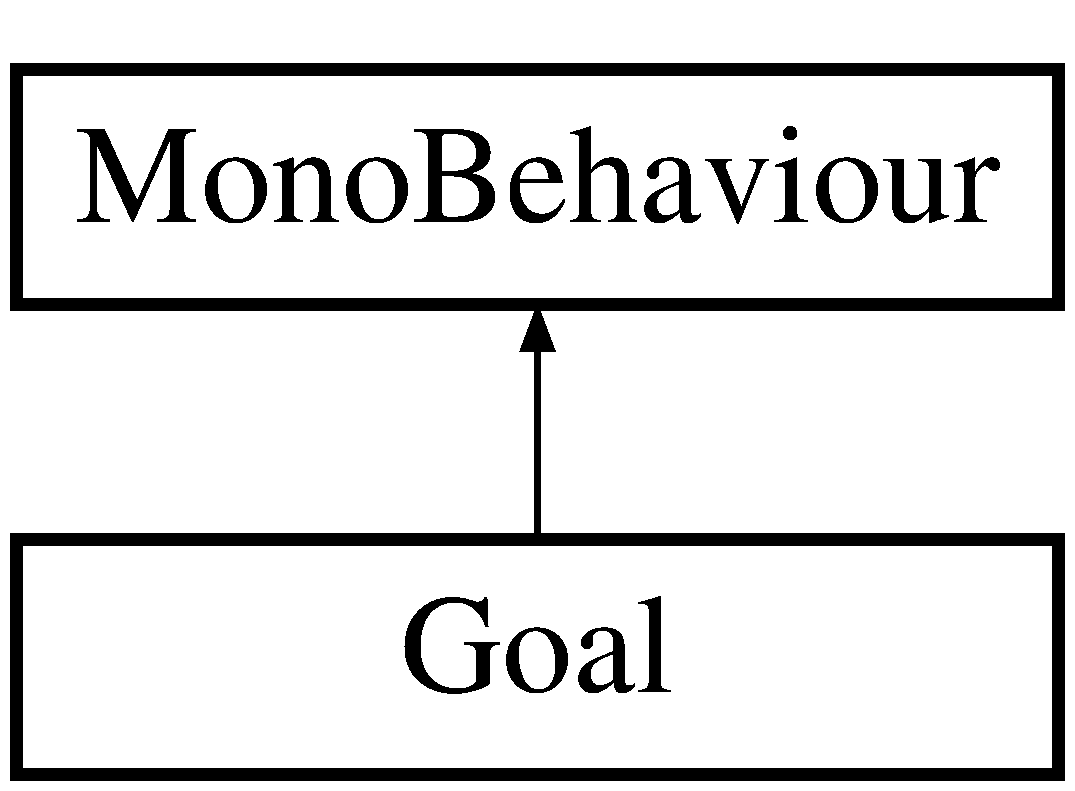
\includegraphics[height=2.000000cm]{class_goal}
\end{center}
\end{figure}


The documentation for this class was generated from the following file\+:\begin{DoxyCompactItemize}
\item 
Assets/\+Code/\+G\+O\+A\+P/Goal.\+cs\end{DoxyCompactItemize}

\hypertarget{class_g_o_a_p}{}\section{G\+O\+A\+P Class Reference}
\label{class_g_o_a_p}\index{G\+O\+A\+P@{G\+O\+A\+P}}
Inheritance diagram for G\+O\+A\+P\+:\begin{figure}[H]
\begin{center}
\leavevmode
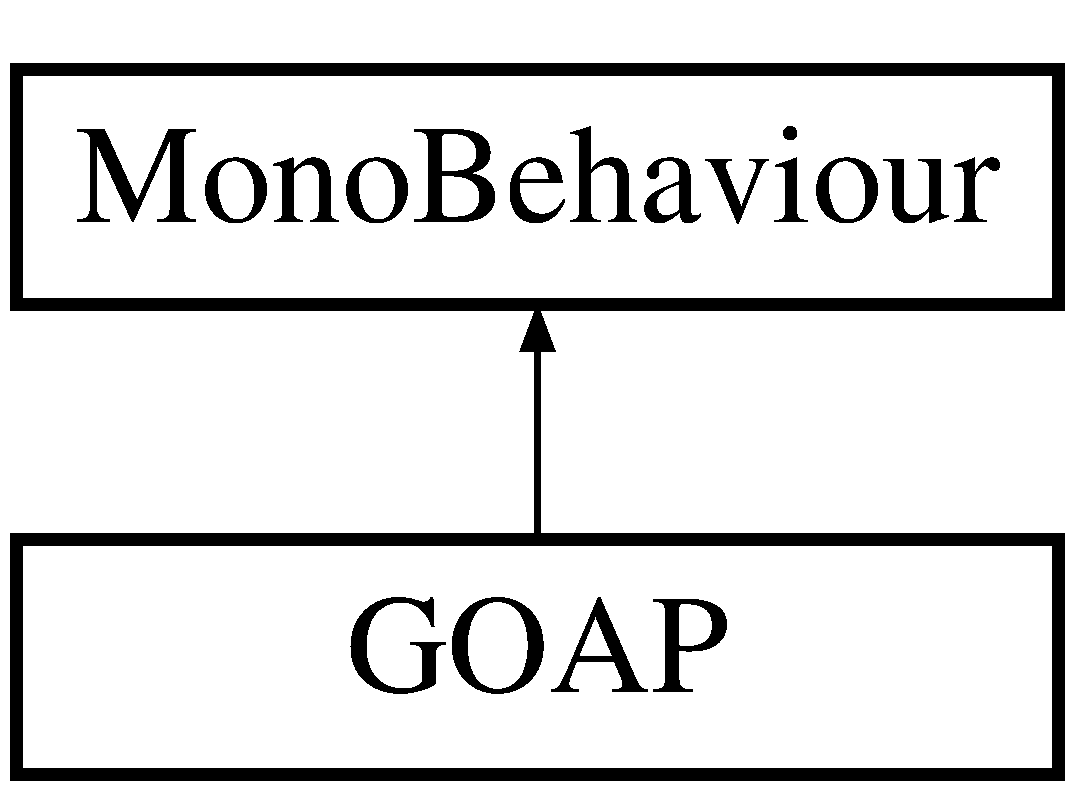
\includegraphics[height=2.000000cm]{class_g_o_a_p}
\end{center}
\end{figure}


The documentation for this class was generated from the following file\+:\begin{DoxyCompactItemize}
\item 
Assets/\+Code/\+G\+O\+A\+P/G\+O\+A\+P.\+cs\end{DoxyCompactItemize}

\hypertarget{class_goap_agent}{}\section{Goap\+Agent Class Reference}
\label{class_goap_agent}\index{Goap\+Agent@{Goap\+Agent}}
Inheritance diagram for Goap\+Agent\+:\begin{figure}[H]
\begin{center}
\leavevmode
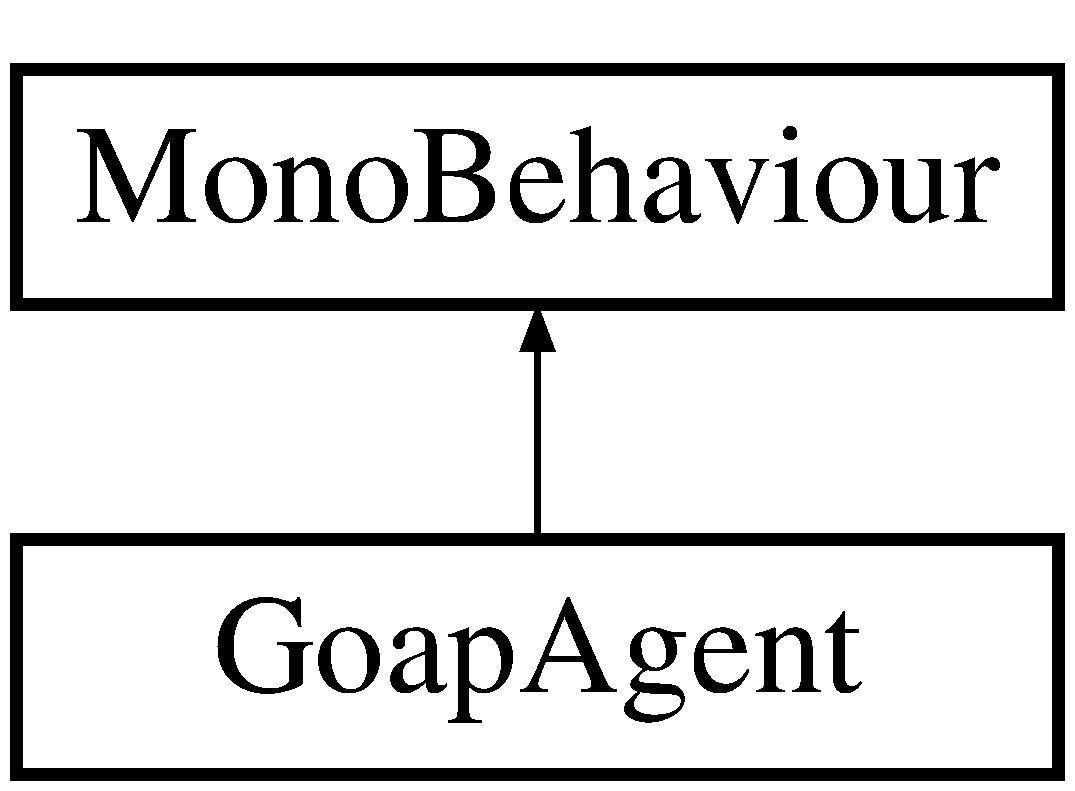
\includegraphics[height=2.000000cm]{class_goap_agent}
\end{center}
\end{figure}
\subsection*{Public Member Functions}
\begin{DoxyCompactItemize}
\item 
\hypertarget{class_goap_agent_a7aa47d1e4c2635f9ad589d31b6277138}{}void {\bfseries add\+Action} (\hyperlink{class_action}{Action} a)\label{class_goap_agent_a7aa47d1e4c2635f9ad589d31b6277138}

\item 
\hypertarget{class_goap_agent_a60a08046c2b464d64638dfeca50ef122}{}\hyperlink{class_action}{Action} {\bfseries get\+Action} (Type action)\label{class_goap_agent_a60a08046c2b464d64638dfeca50ef122}

\item 
\hypertarget{class_goap_agent_a79216e289fd6fcf7625f2358585bbbd5}{}void {\bfseries remove\+Action} (\hyperlink{class_action}{Action} action)\label{class_goap_agent_a79216e289fd6fcf7625f2358585bbbd5}

\end{DoxyCompactItemize}
\subsection*{Static Public Member Functions}
\begin{DoxyCompactItemize}
\item 
\hypertarget{class_goap_agent_a0200bfe84bbe6a5a3672ce943f4af41d}{}static string {\bfseries pretty\+Print} (Hash\+Set$<$ Key\+Value\+Pair$<$ string, object $>$$>$ state)\label{class_goap_agent_a0200bfe84bbe6a5a3672ce943f4af41d}

\item 
\hypertarget{class_goap_agent_a5133fa0a86b32b74a3c69a5f2cf4228b}{}static string {\bfseries pretty\+Print} (Queue$<$ \hyperlink{class_action}{Action} $>$ actions)\label{class_goap_agent_a5133fa0a86b32b74a3c69a5f2cf4228b}

\item 
\hypertarget{class_goap_agent_a05b17d6afd2c0e8291d9bfb2397293cd}{}static string {\bfseries pretty\+Print} (\hyperlink{class_action}{Action}\mbox{[}$\,$\mbox{]} actions)\label{class_goap_agent_a05b17d6afd2c0e8291d9bfb2397293cd}

\item 
\hypertarget{class_goap_agent_ab3bbb156561be37c7fb6631652b843c6}{}static string {\bfseries pretty\+Print} (\hyperlink{class_action}{Action} action)\label{class_goap_agent_ab3bbb156561be37c7fb6631652b843c6}

\end{DoxyCompactItemize}


The documentation for this class was generated from the following file\+:\begin{DoxyCompactItemize}
\item 
Assets/\+Code/\+G\+O\+A\+P/Goap\+Agent.\+cs\end{DoxyCompactItemize}

\hypertarget{class_g_o_a_p_planner}{}\section{G\+O\+A\+P\+Planner Class Reference}
\label{class_g_o_a_p_planner}\index{G\+O\+A\+P\+Planner@{G\+O\+A\+P\+Planner}}


The Planner takes care of providing each agent with a queue of actions that they can perform to achieve their goal. The following code has been copied as is from \href{https://github.com/sploreg/goap/blob/master/Assets/Standard%20Assets/Scripts/AI/GOAP/GoapPlanner.cs}{\tt https\+://github.\+com/sploreg/goap/blob/master/\+Assets/\+Standard\%20\+Assets/\+Scripts/\+A\+I/\+G\+O\+A\+P/\+Goap\+Planner.\+cs}. This has been done as, after an analysys of the code, it was considered impossible to create a version of it that would do the same job in a significantly different way. Therefore the entirety of Brent Owens' code was just copied and refactored to integrate with the existing codebase.  


Inheritance diagram for G\+O\+A\+P\+Planner\+:\begin{figure}[H]
\begin{center}
\leavevmode
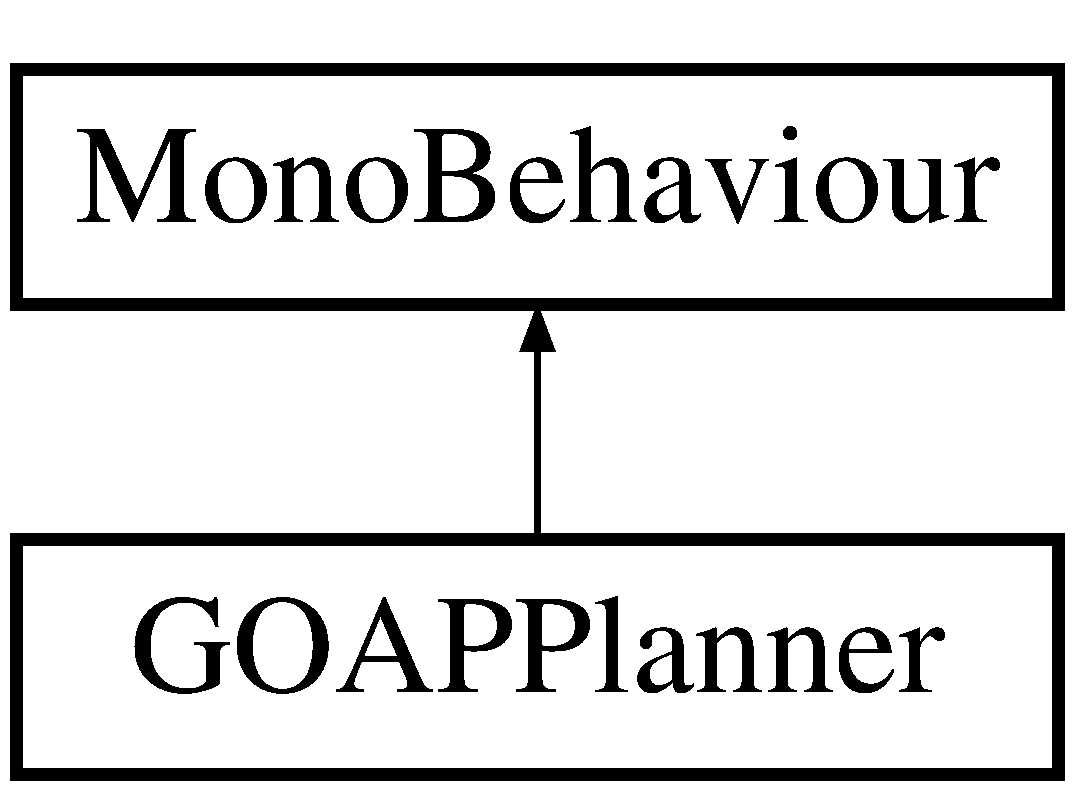
\includegraphics[height=2.000000cm]{class_g_o_a_p_planner}
\end{center}
\end{figure}
\subsection*{Public Member Functions}
\begin{DoxyCompactItemize}
\item 
Queue$<$ \hyperlink{class_action}{Action} $>$ \hyperlink{class_g_o_a_p_planner_a1d2b4333230b1d4ed3a37fedf3fae911}{plan} (Game\+Object agent, Hash\+Set$<$ \hyperlink{class_action}{Action} $>$ available\+Actions, Hash\+Set$<$ Key\+Value\+Pair$<$ string, object $>$$>$ world\+State, Hash\+Set$<$ Key\+Value\+Pair$<$ string, object $>$$>$ goal)
\begin{DoxyCompactList}\small\item\em Tries to find a plan for the given agent. \end{DoxyCompactList}\end{DoxyCompactItemize}


\subsection{Detailed Description}
The Planner takes care of providing each agent with a queue of actions that they can perform to achieve their goal. The following code has been copied as is from \href{https://github.com/sploreg/goap/blob/master/Assets/Standard%20Assets/Scripts/AI/GOAP/GoapPlanner.cs}{\tt https\+://github.\+com/sploreg/goap/blob/master/\+Assets/\+Standard\%20\+Assets/\+Scripts/\+A\+I/\+G\+O\+A\+P/\+Goap\+Planner.\+cs}. This has been done as, after an analysys of the code, it was considered impossible to create a version of it that would do the same job in a significantly different way. Therefore the entirety of Brent Owens' code was just copied and refactored to integrate with the existing codebase. 



\subsection{Member Function Documentation}
\hypertarget{class_g_o_a_p_planner_a1d2b4333230b1d4ed3a37fedf3fae911}{}\index{G\+O\+A\+P\+Planner@{G\+O\+A\+P\+Planner}!plan@{plan}}
\index{plan@{plan}!G\+O\+A\+P\+Planner@{G\+O\+A\+P\+Planner}}
\subsubsection[{plan}]{\setlength{\rightskip}{0pt plus 5cm}Queue$<${\bf Action}$>$ G\+O\+A\+P\+Planner.\+plan (
\begin{DoxyParamCaption}
\item[{Game\+Object}]{agent, }
\item[{Hash\+Set$<$ {\bf Action} $>$}]{available\+Actions, }
\item[{Hash\+Set$<$ Key\+Value\+Pair$<$ string, object $>$$>$}]{world\+State, }
\item[{Hash\+Set$<$ Key\+Value\+Pair$<$ string, object $>$$>$}]{goal}
\end{DoxyParamCaption}
)\hspace{0.3cm}{\ttfamily [inline]}}\label{class_g_o_a_p_planner_a1d2b4333230b1d4ed3a37fedf3fae911}


Tries to find a plan for the given agent. 


\begin{DoxyParams}{Parameters}
{\em agent} & the agent to formulate a plan for\\
\hline
{\em available\+Actions} & a set of available actions for the agent to perform\\
\hline
{\em world\+State} & a set containing the curent state of the world\\
\hline
{\em goal} & the goal to achieve\\
\hline
\end{DoxyParams}
\begin{DoxyReturn}{Returns}
a queue of Actions if a plan is found. Returns Null if a Plan can N\+O\+T be found
\end{DoxyReturn}


The documentation for this class was generated from the following file\+:\begin{DoxyCompactItemize}
\item 
Assets/\+Code/\+G\+O\+A\+P/G\+O\+A\+P\+Planner.\+cs\end{DoxyCompactItemize}

\hypertarget{interface_i_goap}{}\section{I\+Goap Interface Reference}
\label{interface_i_goap}\index{I\+Goap@{I\+Goap}}


Any agent that wants to use \hyperlink{class_g_o_a_p}{G\+O\+A\+P} must implement this interface. It provides information to the \hyperlink{class_g_o_a_p}{G\+O\+A\+P} planner so it can plan what actions to use. It also provides an interface for the planner to give feedback to the Agent and report success/failure.  


\subsection*{Public Member Functions}
\begin{DoxyCompactItemize}
\item 
Hash\+Set$<$ Key\+Value\+Pair$<$ string, object $>$ $>$ \hyperlink{interface_i_goap_afd9fa3eae6e1ee461505b33893637666}{get\+World\+State} ()
\begin{DoxyCompactList}\small\item\em gets a reference to the state of the World \end{DoxyCompactList}\item 
Hash\+Set$<$ Key\+Value\+Pair$<$ string, object $>$ $>$ \hyperlink{interface_i_goap_a33aed8ae113775001f4b2cc1729e5f7a}{create\+Goal\+State} ()
\begin{DoxyCompactList}\small\item\em Provides a new \hyperlink{class_goal}{Goal} to the Planner \end{DoxyCompactList}\item 
void \hyperlink{interface_i_goap_a2654ec9b902683ce5f5fe31434889ea0}{plan\+Failed} (Hash\+Set$<$ Key\+Value\+Pair$<$ string, object $>$$>$ failed\+Goal)
\begin{DoxyCompactList}\small\item\em If a plan failed to be created, a new one will be tried excluding the failed goal from the creation process \end{DoxyCompactList}\item 
void \hyperlink{interface_i_goap_a5aa7548d02bfd0f8f0143c15b4282cd0}{plan\+Found} (Hash\+Set$<$ Key\+Value\+Pair$<$ string, object $>$$>$ goal, Queue$<$ \hyperlink{class_action}{Action} $>$ actions)
\begin{DoxyCompactList}\small\item\em If a plan was found, a queue of Actions is provided for the requested \hyperlink{class_goal}{Goal} \end{DoxyCompactList}\item 
void \hyperlink{interface_i_goap_a62899286cd2362e0d870c688a98ccdd6}{actions\+Finished} ()
\begin{DoxyCompactList}\small\item\em decides what happens once all the actions are completed \end{DoxyCompactList}\item 
void \hyperlink{interface_i_goap_aee6419a123508fe7a8696ae9fde698f8}{plan\+Aborted} (\hyperlink{class_action}{Action} aborter)
\begin{DoxyCompactList}\small\item\em If one of the actions made the plan be aborted, this function gets called \end{DoxyCompactList}\item 
bool \hyperlink{interface_i_goap_a32aadeff3002e72b2e575cb21f527ec0}{move\+Agent} (\hyperlink{class_action}{Action} next\+Action)
\begin{DoxyCompactList}\small\item\em this method gets called during update and takes care of moving the Agent to his next destination \end{DoxyCompactList}\end{DoxyCompactItemize}


\subsection{Detailed Description}
Any agent that wants to use \hyperlink{class_g_o_a_p}{G\+O\+A\+P} must implement this interface. It provides information to the \hyperlink{class_g_o_a_p}{G\+O\+A\+P} planner so it can plan what actions to use. It also provides an interface for the planner to give feedback to the Agent and report success/failure. 



\subsection{Member Function Documentation}
\hypertarget{interface_i_goap_a62899286cd2362e0d870c688a98ccdd6}{}\index{I\+Goap@{I\+Goap}!actions\+Finished@{actions\+Finished}}
\index{actions\+Finished@{actions\+Finished}!I\+Goap@{I\+Goap}}
\subsubsection[{actions\+Finished}]{\setlength{\rightskip}{0pt plus 5cm}void I\+Goap.\+actions\+Finished (
\begin{DoxyParamCaption}
{}
\end{DoxyParamCaption}
)}\label{interface_i_goap_a62899286cd2362e0d870c688a98ccdd6}


decides what happens once all the actions are completed 

\hypertarget{interface_i_goap_a33aed8ae113775001f4b2cc1729e5f7a}{}\index{I\+Goap@{I\+Goap}!create\+Goal\+State@{create\+Goal\+State}}
\index{create\+Goal\+State@{create\+Goal\+State}!I\+Goap@{I\+Goap}}
\subsubsection[{create\+Goal\+State}]{\setlength{\rightskip}{0pt plus 5cm}Hash\+Set$<$Key\+Value\+Pair$<$string, object$>$ $>$ I\+Goap.\+create\+Goal\+State (
\begin{DoxyParamCaption}
{}
\end{DoxyParamCaption}
)}\label{interface_i_goap_a33aed8ae113775001f4b2cc1729e5f7a}


Provides a new \hyperlink{class_goal}{Goal} to the Planner 

\begin{DoxyReturn}{Returns}
the new \hyperlink{class_goal}{Goal} created
\end{DoxyReturn}
\hypertarget{interface_i_goap_afd9fa3eae6e1ee461505b33893637666}{}\index{I\+Goap@{I\+Goap}!get\+World\+State@{get\+World\+State}}
\index{get\+World\+State@{get\+World\+State}!I\+Goap@{I\+Goap}}
\subsubsection[{get\+World\+State}]{\setlength{\rightskip}{0pt plus 5cm}Hash\+Set$<$Key\+Value\+Pair$<$string, object$>$ $>$ I\+Goap.\+get\+World\+State (
\begin{DoxyParamCaption}
{}
\end{DoxyParamCaption}
)}\label{interface_i_goap_afd9fa3eae6e1ee461505b33893637666}


gets a reference to the state of the World 

\begin{DoxyReturn}{Returns}
a Hash Set containing the state of the World
\end{DoxyReturn}
\hypertarget{interface_i_goap_a32aadeff3002e72b2e575cb21f527ec0}{}\index{I\+Goap@{I\+Goap}!move\+Agent@{move\+Agent}}
\index{move\+Agent@{move\+Agent}!I\+Goap@{I\+Goap}}
\subsubsection[{move\+Agent}]{\setlength{\rightskip}{0pt plus 5cm}bool I\+Goap.\+move\+Agent (
\begin{DoxyParamCaption}
\item[{{\bf Action}}]{next\+Action}
\end{DoxyParamCaption}
)}\label{interface_i_goap_a32aadeff3002e72b2e575cb21f527ec0}


this method gets called during update and takes care of moving the Agent to his next destination 


\begin{DoxyParams}{Parameters}
{\em next\+Action} & the \hyperlink{class_action}{Action} to perform when the destination is reached\\
\hline
\end{DoxyParams}
\begin{DoxyReturn}{Returns}
true if destination has been reached
\end{DoxyReturn}
\hypertarget{interface_i_goap_aee6419a123508fe7a8696ae9fde698f8}{}\index{I\+Goap@{I\+Goap}!plan\+Aborted@{plan\+Aborted}}
\index{plan\+Aborted@{plan\+Aborted}!I\+Goap@{I\+Goap}}
\subsubsection[{plan\+Aborted}]{\setlength{\rightskip}{0pt plus 5cm}void I\+Goap.\+plan\+Aborted (
\begin{DoxyParamCaption}
\item[{{\bf Action}}]{aborter}
\end{DoxyParamCaption}
)}\label{interface_i_goap_aee6419a123508fe7a8696ae9fde698f8}


If one of the actions made the plan be aborted, this function gets called 


\begin{DoxyParams}{Parameters}
{\em aborter} & the \hyperlink{class_action}{Action} that caused the plan to get aborted\\
\hline
\end{DoxyParams}
\hypertarget{interface_i_goap_a2654ec9b902683ce5f5fe31434889ea0}{}\index{I\+Goap@{I\+Goap}!plan\+Failed@{plan\+Failed}}
\index{plan\+Failed@{plan\+Failed}!I\+Goap@{I\+Goap}}
\subsubsection[{plan\+Failed}]{\setlength{\rightskip}{0pt plus 5cm}void I\+Goap.\+plan\+Failed (
\begin{DoxyParamCaption}
\item[{Hash\+Set$<$ Key\+Value\+Pair$<$ string, object $>$$>$}]{failed\+Goal}
\end{DoxyParamCaption}
)}\label{interface_i_goap_a2654ec9b902683ce5f5fe31434889ea0}


If a plan failed to be created, a new one will be tried excluding the failed goal from the creation process 


\begin{DoxyParams}{Parameters}
{\em failed\+Goal} & the goal we failed to achieve\\
\hline
\end{DoxyParams}
\hypertarget{interface_i_goap_a5aa7548d02bfd0f8f0143c15b4282cd0}{}\index{I\+Goap@{I\+Goap}!plan\+Found@{plan\+Found}}
\index{plan\+Found@{plan\+Found}!I\+Goap@{I\+Goap}}
\subsubsection[{plan\+Found}]{\setlength{\rightskip}{0pt plus 5cm}void I\+Goap.\+plan\+Found (
\begin{DoxyParamCaption}
\item[{Hash\+Set$<$ Key\+Value\+Pair$<$ string, object $>$$>$}]{goal, }
\item[{Queue$<$ {\bf Action} $>$}]{actions}
\end{DoxyParamCaption}
)}\label{interface_i_goap_a5aa7548d02bfd0f8f0143c15b4282cd0}


If a plan was found, a queue of Actions is provided for the requested \hyperlink{class_goal}{Goal} 


\begin{DoxyParams}{Parameters}
{\em goal} & the requested \hyperlink{class_goal}{Goal}\\
\hline
{\em actions} & the queue of Actions to be executed to achieve the \hyperlink{class_goal}{Goal}\\
\hline
\end{DoxyParams}


The documentation for this interface was generated from the following file\+:\begin{DoxyCompactItemize}
\item 
Assets/\+Code/\+G\+O\+A\+P/I\+Goap.\+cs\end{DoxyCompactItemize}

%--- End generated contents ---

% Index
\backmatter
\newpage
\phantomsection
\clearemptydoublepage
\addcontentsline{toc}{chapter}{Index}
\printindex

\end{document}
